\RequirePackage{currfile}
\documentclass[12pt]{beamer}
\usepackage[utf8]{inputenc}
\usepackage[spanish]{babel}
\usepackage{standalone}
\usepackage{color}
\usepackage{siunitx}
\usepackage{hyperref}
\usepackage[outdir=./]{epstopdf}
%\hypersetup{colorlinks,linkcolor=,urlcolor=blue}
%\hypersetup{colorlinks,urlcolor=blue}
\usepackage{xcolor,soul}
\usepackage{etoolbox}
\usepackage{amsmath}
\usepackage{amsthm}
\usepackage{mathtools}
\usepackage{tcolorbox}
\usepackage{physics}
\usepackage{multicol}
\usepackage{bookmark}
\usepackage{longtable}
\usepackage{listings}
\usepackage{cancel}
\usepackage{wrapfig}
\usepackage{empheq}
\usepackage{graphicx}
\usepackage{tikz}
\usetikzlibrary{calc, patterns, matrix, backgrounds, decorations,shapes, arrows.meta}
\usepackage[autostyle,spanish=mexican]{csquotes}
\usepackage[os=win]{menukeys}
\usepackage{pifont}
\usepackage{pbox}
\usepackage{bm}
\usepackage{caption}
\captionsetup{font=scriptsize,labelfont=scriptsize}
%\usepackage[sfdefault]{roboto}  %% Option 'sfdefault' only if the base font of the document is to be sans serif

%Sección de definición de colores
\definecolor{ao}{rgb}{0.0, 0.5, 0.0}
\definecolor{bisque}{rgb}{1.0, 0.89, 0.77}
\definecolor{amber}{rgb}{1.0, 0.75, 0.0}
\definecolor{armygreen}{rgb}{0.29, 0.33, 0.13}
\definecolor{alizarin}{rgb}{0.82, 0.1, 0.26}
\definecolor{cadetblue}{rgb}{0.37, 0.62, 0.63}
\definecolor{deepblue}{rgb}{0,0,0.5}
\definecolor{brown}{rgb}{0.59, 0.29, 0.0}
\definecolor{OliveGreen}{rgb}{0,0.25,0}
\definecolor{mycolor}{rgb}{0.122, 0.435, 0.698}

\newcommand*{\boxcolor}{orange}
\makeatletter
\newcommand{\boxedcolor}[1]{\textcolor{\boxcolor}{%
\tikz[baseline={([yshift=-1ex]current bounding box.center)}] \node [rectangle, minimum width=1ex, thick, rounded corners,draw] {\normalcolor\m@th$\displaystyle#1$};}}
 \makeatother

\newtcbox{\mybox}{on line,
  colframe=mycolor,colback=mycolor!10!white,
  boxrule=0.5pt,arc=4pt,boxsep=0pt,left=6pt,right=6pt,top=6pt,bottom=6pt}

\usefonttheme[onlymath]{serif}
%Sección de definición de nuevos comandos

\newcommand*{\TitleParbox}[1]{\parbox[c]{1.75cm}{\raggedright #1}}%
\newcommand{\python}{\texttt{python}}
\newcommand{\textoazul}[1]{\textcolor{blue}{#1}}
\newcommand{\azulfuerte}[1]{\textcolor{blue}{\textbf{#1}}}
\newcommand{\funcionazul}[1]{\textcolor{blue}{\textbf{\texttt{#1}}}}
\newcommand{\ptilde}[1]{\ensuremath{{#1}^{\prime}}}
\newcommand{\stilde}[1]{\ensuremath{{#1}^{\prime \prime}}}
\newcommand{\ttilde}[1]{\ensuremath{{#1}^{\prime \prime \prime}}}
\newcommand{\ntilde}[2]{\ensuremath{{#1}^{(#2)}}}
\renewcommand{\arraystretch}{1.5}

\newcounter{saveenumi}
\newcommand{\seti}{\setcounter{saveenumi}{\value{enumi}}}
\newcommand{\conti}{\setcounter{enumi}{\value{saveenumi}}}
\renewcommand{\rmdefault}{cmr}% cmr = Computer Modern Roman

\linespread{1.5}

\usefonttheme{professionalfonts}
%\usefonttheme{serif}
\DeclareGraphicsExtensions{.pdf,.png,.jpg}


%Sección para el tema de beamer, con el theme, usercolortheme y sección de footers
\mode<presentation>
{
  \usetheme{CambridgeUS}
  
  %\useoutertheme{infolines}
  \useoutertheme{default}
  \usecolortheme{beaver}
  \setbeamercovered{invisible}
  % or whatever (possibly just delete it)
  \setbeamertemplate{section in toc}[sections numbered]
  \setbeamertemplate{subsection in toc}[subsections numbered]
  \setbeamertemplate{subsection in toc}{\leavevmode\leftskip=3.2em\rlap{\hskip-2em\inserttocsectionnumber.\inserttocsubsectionnumber}\inserttocsubsection\par}
  \setbeamercolor{section in toc}{fg=blue}
  \setbeamercolor{subsection in toc}{fg=blue}
  \setbeamercolor{frametitle}{fg=blue}
  \setbeamertemplate{caption}[numbered]

  \setbeamertemplate{footline}
  \beamertemplatenavigationsymbolsempty
  \setbeamertemplate{headline}{}
}

\makeatletter
\setbeamercolor{section in foot}{bg=gray!30, fg=black!90!orange}
\setbeamercolor{subsection in foot}{bg=blue!30!yellow, fg=red}
\setbeamertemplate{footline}
{
  \leavevmode%
  \hbox{%
  \begin{beamercolorbox}[wd=.333333\paperwidth,ht=2.25ex,dp=1ex,center]{section in foot}%
    \usebeamerfont{section in foot} \insertsection
  \end{beamercolorbox}}%
  \begin{beamercolorbox}[wd=.333333\paperwidth,ht=2.25ex,dp=1ex,center]{subsection in foot}%
    \usebeamerfont{subsection in foot}  \insertsubsection
  \end{beamercolorbox}%
  \begin{beamercolorbox}[wd=.333333\paperwidth,ht=2.25ex,dp=1ex,right]{date in head/foot}%
    \usebeamerfont{date in head/foot} \insertshortdate{} \hspace*{2em}
    \insertframenumber{} / \inserttotalframenumber \hspace*{2ex} 
  \end{beamercolorbox}}%
  \vskip0pt%
\makeatother  

\makeatletter
\patchcmd{\beamer@sectionintoc}
  {\vfill}
  {\vskip\itemsep}
  {}
  {}
\makeatother


\title{\large{Introducción}}
\subtitle{Tema 2 - Método de separación de variables}
\author{M. en C. Gustavo Contreras Mayén}
\date{}
\institute{Facultad de Ciencias - UNAM}
\titlegraphic{
\includegraphics[width=1.75cm]{../Imagenes/escudo-facultad-ciencias}\hspace*{4.75cm}~%
   
\includegraphics[width=1.75cm]{../Imagenes/escudo-unam}
}
\setbeamertemplate{navigation symbols}{}
\begin{document}
\maketitle
\fontsize{14}{14}\selectfont
\spanishdecimal{.}
\section*{Contenido}
\frame{\tableofcontents[currentsection, hideallsubsections]}
\section{Ecuaciones Diferenciales Parciales}
\frame{\tableofcontents[currentsection, hideothersubsections]}
\subsection{Introducción}
\begin{frame}
\frametitle{Solución de las EDP}
Una vez que se ha realizado la formulación de una EDP el siguiente paso es resolver la ecuación, en un primer momento podemos considerar la solución general de la EDP, entonces en vez de constantes arbitrarias aparecen funciones arbitrarias.
\\
\bigskip
\pause
Por ejemplo, la solución general de $u_{xy} = 0$ es $u(x, y) = G(x) + F (y)$ donde $G$, $F$ son funciones arbitrarias.
\end{frame}
\begin{frame}
\frametitle{Solución de las EDP}
Dado que se quieren resolver problemas específicos, hay que estudiar el tipo de condiciones que hay que imponer para garantizar \emph{la unicidad} de la solución.
\end{frame}
\begin{frame}
\frametitle{Solución de las EDP}
Como se revisó en la presentación anterior, tenemos una clasificación con tres tipos de ecuaciones (parabólica, hiperbólica y elíptica) a continuación presentamos un posible tipo de condiciones de frontera (CDF) que se pueden presentar.
\end{frame}
\section{Condiciones de frontera}
\frame[allowframebreaks]{\tableofcontents[currentsection, hideothersubsections]}
\subsection{EDP Parabólica}
\begin{frame}
\frametitle{Ecuación de calor}
Consideremos la ecuación del calor
\begin{align*}
u_{t} =  \alpha^{2} \,  u_{xx}
\end{align*}
En este caso se trabajará con un problema unidimensional, es decir, la transmisión del calor a lo largo de una barra de longitud $L$.
\end{frame}
\begin{frame}
\frametitle{Condiciones de frontera}
Para que el problema tenga solución se debe de especificar la distribución inicial de temperatura de la barra, es decir, hay que dar una función $\varphi (x)$ de modo que la distribución inicial de temperatura es:
\begin{align}
u(x, 0) = \alpha (x)
\label{eq:ecuacion_06_02_02}
\end{align}
que en analogía con las ODE, tiene sentido llamar tal condición una \emph{condición inicial}.
\end{frame}
\begin{frame}
\frametitle{Condiciones de frontera}
A su vez, como la barra tiene una longitud finita, hay que especificar la interacción de los extremos de la barra con el medio ambiente. Tales condiciones se conocen como \emph{condiciones de frontera}.
\par
Para los problemas de una dimensión hay tres tipos de condiciones de frontera usuales, aunque solo se estudiarán las primeras dos en esta revisión:
\end{frame}
\begin{frame}
\frametitle{Condiciones de frontera}
\setbeamercolor{item projected}{bg=blue!70!black,fg=yellow}
\setbeamertemplate{enumerate items}[circle]
\begin{enumerate}
\item \textbf{Condición de Dirichlet}: Consiste en especificar la temperatura en los extremos de la barra en todo instante, es decir, dar dos funciones $f(t)$ y $g(t)$ de modo que:
\begin{align}
u(0, t) = f (t)  \hspace{1cm} u(L, t) = g(t)
\label{eq:ecuacion_06_02_03}    
\end{align}
Estas son las condiciones de tipo Dirichlet.
\seti
\end{enumerate}
\end{frame}
\begin{frame}
\frametitle{Condiciones de frontera}
\setbeamercolor{item projected}{bg=blue!70!black,fg=yellow}
\setbeamertemplate{enumerate items}[circle]
\begin{enumerate}
\conti
\item \textbf{Condición de Neumann}: Consiste en especificar la derivada de la temperatura en los extremos de la barra, es decir, especificar el flujo de calor en los extremos de la barra:
\begin{align}
u_{x}(0,t) = f(t) \hspace{1cm} u_{x}(L,t) = g(t)
\label{eq:ecuacion_06_02_04}    
\end{align}
Estas son las condiciones de tipo Neumann.
\seti
\end{enumerate}
\end{frame}
\begin{frame}
\frametitle{Condiciones de frontera}
\setbeamercolor{item projected}{bg=blue!70!black,fg=yellow}
\setbeamertemplate{enumerate items}[circle]
\begin{enumerate}
\conti
\item \textbf{Condiciones mixtas (de Robin)}: Consiste en especificar una combinación de $u$ y de $u_{x}$ en los extremos de la barra.
\end{enumerate}
\end{frame}
\subsection{EDP Elíptica}
\begin{frame}
\frametitle{La ecuación de trabajo}
Sea la ecuación de Laplace:
\begin{align*}
u_{xx} + u_{yy} = 0
\end{align*}
Se puede interpretar como la ecuación de un potencial electrostático sobre una región del plano $xy$ o bien la distribución de temperatura en el caso estacionario para una placa o una región del plano $xy$.
\end{frame}
\begin{frame}
\frametitle{Condiciones de la EDP}
En este caso no hay que especificar condiciones iniciales pues la función no depende del tiempo. Se estudiarán dos tipos de condiciones:
\end{frame}
\begin{frame}
\frametitle{Condiciones de la EDP}
\setbeamercolor{item projected}{bg=blue!70!black,fg=yellow}
\setbeamertemplate{enumerate items}[circle]
\begin{enumerate}
\item \textbf{Condición de Dirichlet}: Si se trabaja sobre una lámina rectangular $0 < x < a$ y $0 < y < b$ las condiciones de Dirichlet consisten en especificar los valores de la temperatura (o el potencial) sobre todos los lados, es decir:
\seti
\end{enumerate}
\end{frame}
\begin{frame}
\frametitle{Condiciones de la EDP}
\begin{align}
\begin{aligned}
u(0, y) &= f_{1}(y) \hspace{1cm} u(a, y) = f_{2}(y) \\
u(x, 0) &= g_{1}(x) \hspace{1cm} u(x, b) = g_{2}(x)
\end{aligned}
\label{eq:ecuacion_06_02_05}
\end{align}
\end{frame}
\begin{frame}
\frametitle{Condiciones de la EDP}
\setbeamercolor{item projected}{bg=blue!70!black,fg=yellow}
\setbeamertemplate{enumerate items}[circle]
\begin{enumerate}
\conti    
\item \textbf{Condiciones Mixtas}: Para los lados de la placa se toman dos de las condiciones de Dirichlet y las otras dos de Neumann, por ejemplo:
\begin{align}
\begin{aligned}
u_{y}(0, y) &= f_{1}(y) \hspace{1cm} u_{y}(a, y) = f_{2}(y) \\
u(x, 0) &= g_{1}(x) \hspace{1cm} u(x, b) = g_{2}(x)
\end{aligned}
\label{eq:ecuacion_06_01_06}
\end{align}
\end{enumerate}
\end{frame}
\subsection{EDP Hiperbólica}
\begin{frame}
\frametitle{La ecuación de trabajo}
Consideremos ahora la ecuación de onda
\begin{align*}
u_{tt} = v^{2} \, u_{xx}
\end{align*}
En este caso se considera una cuerda de longitud $L$. 
\end{frame}
\begin{frame}
\frametitle{Condiciones iniciales}
Como la ecuación es de segundo orden en el tiempo, tiene sentido esperar que haya que especificar la posición inicial de la cuerda así como su velocidad inicial, es decir, proporcionar las condiciones iniciales (CI):
\begin{align}
u(x, 0) = \phi (x) \hspace{1cm} u_{t}(x, 0) = \psi (x)
\label{eq:ecuacion_06_02_07}
\end{align}
\end{frame}
\begin{frame}
\frametitle{Condiciones de frontera}
A su vez, hay que especificar como se relaciona la cuerda con su frontera y nuevamente se van a estudiar las condiciones de Dirichlet y de Neumann:
\end{frame}
\begin{frame}
\frametitle{Condiciones de frontera}
\setbeamercolor{item projected}{bg=blue!70!black,fg=yellow}
\setbeamertemplate{enumerate items}[circle]
\begin{enumerate}
\item \textbf{Condición de Dirichlet}: Se especifica la posición de los extremos de la cuerda, es decir:
\begin{align}
u(0, t) = f (t) \hspace{1cm} u(L, t) = g(t)
\label{eq:ecuacion_06_02_08}   
\end{align}
\seti
\end{enumerate}
\end{frame}
\begin{frame}
\frametitle{Condiciones de frontera}
\setbeamercolor{item projected}{bg=blue!70!black,fg=yellow}
\setbeamertemplate{enumerate items}[circle]
\begin{enumerate}
\conti
\item \textbf{Condición de Neumann}: Se especifica la forma en que se están \enquote{jalando} los extremos de la cuerda, es decir:
\begin{align}
u_{x}(0, t) = f(t) \hspace{1cm} u_{x}(L,t) = g(t)
\label{eq:ecuacion_06_02_09}    
\end{align}
\end{enumerate}
\end{frame}
\begin{frame}
\frametitle{Consideraciones}
Como se veremos más adelante, el \emph{método de separación de variables} consiste en suponer que la solución depende como un producto de funciones, cada una de las cuales depende exclusivamente de una de las variables independientes.
\end{frame}
\begin{frame}
\frametitle{Consideraciones}
Para que tenga éxito el método, se ocupará que varias de las condiciones de frontera estén igualadas a cero, de forma que se utilicen para restringir las soluciones a las ecuaciones diferenciales ordinarias que aparecen.
\end{frame}
\begin{frame}
\frametitle{Consideraciones}
Luego, dado que las ecuaciones son lineales se propone por el principio de superposición una combinación lineal (de hecho una serie en la mayoría de los casos) de tales soluciones y las constantes que aparecen se hallan tomando el desarrollo de Fourier de las otras condiciones iniciales o de frontera que todavía no se han utilizado.
\end{frame}
\section{Método de separación de variables}
\frame[allowframebreaks]{\tableofcontents[currentsection, hideothersubsections]}
\subsection{Descripción}
\begin{frame}
\frametitle{El método}
El método de separación de variables es una de las técnicas más antiguas para resolver problemas de valores con condiciones iniciales y se aplica en problemas donde:
\setbeamercolor{item projected}{bg=blue!70!black,fg=yellow}
\setbeamertemplate{enumerate items}[circle]
\begin{enumerate}
\item La EDP es lineal y homogénea (no necesariamente con coeficientes constantes).
\seti
\end{enumerate}
\end{frame}
\begin{frame}
\frametitle{El método}
\setbeamercolor{item projected}{bg=blue!70!black,fg=yellow}
\setbeamertemplate{enumerate items}[circle]
\begin{enumerate}
\item Las condiciones de frontera tienen la forma:
\begin{align*}
\alpha \, u_{x} (0, t) + \beta \, u(0, t) &= 0 \\
\gamma \, u_{x} (1, t) + \delta \, u(1, t) &= 0
\end{align*}
donde $\alpha, \beta, \gamma, \delta$ son constantes (las condiciones de frontera de esta forma se denominan \textbf{condiciones de frontera lineales homogéneas}).
\end{enumerate}
\end{frame}
\begin{frame}
\frametitle{El método}
Como referencia histórica, este método se remonta a la época de Joseph Fourier (de hecho, ocasionalmente se le llama \emph{método de Fourier}) y es probablemente el método de solución más utilizado (cuando corresponde).
\\
\bigskip
\pause
En lugar de mostrar cómo funciona el método en general, apliquémoslo a un problema específico.
\end{frame}
\subsection{Planteamiento del problema}
\begin{frame}
\frametitle{La ecuación de calor}
Considera el siguiente problema de valores iniciales con la ecuación de calor:
\\
\bigskip
Ecuación diferencial:
\begin{align*}
\addtolength{\fboxsep}{5pt}\boxed{ u_{t} = \alpha^{2} \, u_{xx}, \hspace{1cm} 0 < x < L,\hspace{0.5cm} 0 < t < \infty}
\end{align*}
\end{frame}
\begin{frame}
\frametitle{Condiciones de frontera}
Condiciones de frontera (CDF):
\begin{align*}
\addtolength{\fboxsep}{5pt}\boxed{
\begin{cases}
u(0, t) = 0 \\
u(L, t) = 0
\end{cases}
\hspace{1.5cm}
0 < t < \infty }
\end{align*}
\end{frame}
\begin{frame}
\frametitle{Condiciones iniciales}
Condiciones iniciales (CI):
\begin{align*}
\addtolength{\fboxsep}{5pt}\boxed{
u(x, 0) = \phi (x) \hspace{1.5cm} 0 \leq x \leq L
}
\end{align*}
\end{frame}
\begin{frame}
\frametitle{Antes de resolver}
Antes de revisar el método de separación de variables, pensemos primero en nuestro problema: Aquí tenemos una varilla finita de longitud $L$ donde la temperatura en los extremos se fija en cero (supongamos que es un problema de temperatura donde cero significa tantos grados).
\end{frame}
\begin{frame}
\frametitle{Antes de resolver}
También se nos dan datos sobre el problema en forma de condición inicial; nuestro objetivo es encontrar la temperatura $u (x, t)$ en puntos posteriores en el tiempo.
\\
\bigskip
\pause
Ahora veamos una descripción general.
\end{frame}
\subsection{La técnica}
\begin{frame}
\frametitle{Suposición de una solución}
El método de separación de variables supone la existencia de soluciones sencillas de una EDP de la forma
\begin{align*}
u(x, t) =  X(x) \, T(t)
\end{align*}
donde $X (x)$ es alguna función de $x$ y $T (t)$ es alguna función de $t$.
\end{frame}
\begin{frame}
\frametitle{Soluciones al problema}
Las soluciones son sencillas porque cualquier temperatura $u (x, t)$ de esta forma conservará su \enquote{forma} básica para diferentes valores de tiempo $t$, como podemos ver en la figura (\ref{fig:figura_separacion_variables_01})
\begin{figure}[H]
    \centering
    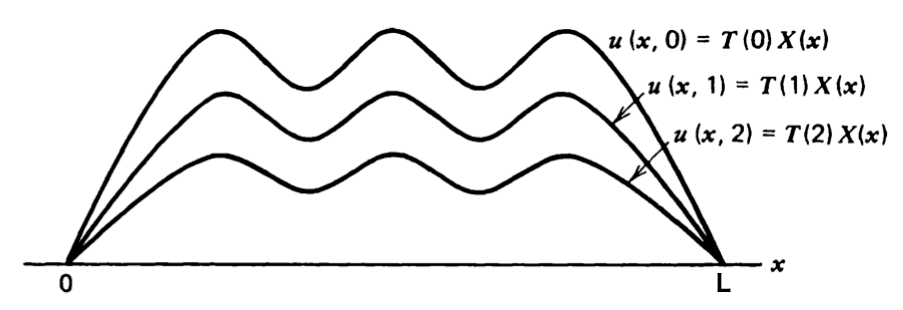
\includegraphics[scale=0.25]{Imagenes/Separacion_Variables_01.png}
    \caption{Gráfica de $X(x)$ y $T(t)$ para distintos valores de $t$.}
    \label{fig:figura_separacion_variables_01}
\end{figure}
\end{frame}
\begin{frame}
\frametitle{Soluciones fundamentales}
La idea general que tenemos nos plantea la posibilidad de encontrar un número infinito de estas soluciones a la EDP (que al mismo tiempo también satisfacen las condiciones de frontera).
\end{frame}
\begin{frame}
\frametitle{Soluciones fundamentales}
Estas funciones simples
\begin{align*}
u_{n} (t) = X_{n} (x) \, T_{n}(t)
\end{align*}
se les denomina \textbf{soluciones fundamentales}, son las componentes básicas de nuestro problema, y de la solución $u (x, t)$ que estamos buscando.
\end{frame}
\begin{frame}
\frametitle{Soluciones al problema}
Sumando las soluciones fundamentales $X_{n}(x) \, T_{n} (t)$ de tal manera que la suma resultante
\begin{align*}
\sum_{n=1}^{\infty} A_{n} \, X_{n} (x) \, T_{n} (t)
\end{align*}
satisface las condiciones iniciales.
\end{frame}
\begin{frame}
\frametitle{Soluciones al problema}
Dado que esta suma aún satisface la EDP y las CDF, ahora tenemos la solución a nuestro problema.
\\
\bigskip
\pause
Veamos a detalle el método de separación de variables.
\end{frame}
\subsection{Paso 1}
\begin{frame}
\frametitle{Encontrar las soluciones elementales de la EDP}
Nos interesa encontrar la función $u(x, t)$ que satisfaga las siguientes condiciones:
\begin{align*}
\mbox{EDP} \hspace{1cm} &u_{t} = \alpha^{2} \, u_{xx} \hspace{0.5cm} 0 < x < L, \hspace{0.3cm} 0 < t < \infty \\[0.5em] 
\mbox{CDF} \hspace{1cm} &\begin{cases}
    u(0, t) = 0 \\
    u(L, t) = 0
    \end{cases}
    \hspace{1cm}
    0 < t < \infty \\[0.5em]
CI \hspace{1cm} & u(x, 0) = \phi (x) \hspace{1cm} 0 \leq x \leq L
\end{align*}
\end{frame}
\begin{frame}
\frametitle{Sustituir la solución propuesta}
Para comenzar, buscamos soluciones de la forma $u (x, t) = X(x) \, T (t)$ sustituyendo $X (x) \, T (t)$ en la EDP y resolvemos para  $X (x) \, T (t)$. Haciendo esta sustitución obtenemos:
\begin{align*}
X(x) \, T (t) = \alpha^{2} \, X (x) \, T(t)
\end{align*}
\end{frame}
\begin{frame}
\frametitle{Sustituir la solución propuesta}
La parte que hace todo el trabajo es la siguiente: si \emph{dividimos} cada lado de esta ecuación por $\alpha^{2} \, X(x) \, T(t)$, tenemos que:
\begin{align*}
\dfrac{T^{\prime} (t)}{\alpha^{2} \, T(t)} = \dfrac{X^{\prime \prime} (x)}{X(x)}
\end{align*}
para obtener lo que se conoce como \emph{variables separables}, es decir, la expresión del lado izquierdo de la igualdad depende solo de $t$, mientras que la expresión del lado derecho, depende solo de $x$.
\end{frame}
\begin{frame}
\frametitle{Constante de separación}
Dado que $x$ y $t$ son independientes entre sí, cada lado debe ser una constante fija (digamos $k$),  por tanto podemos escribir:
\begin{align*}
\dfrac{T^{\prime}}{\alpha^{2} \, T} = \dfrac{X^{\prime \prime}}{X} = k
\end{align*}
\end{frame}
\begin{frame}
\frametitle{Sistema de EDO}
De manera equivalente
\begin{align*}
T^{\prime} - k \, \alpha^{2} \, T &= 0 \\[0.5em]
X^{\prime \prime} - k \, X &= 0
\end{align*}
\\
\bigskip
\pause
Entonces, ahora podemos resolver cada uno de estas dos EDO, para luego multiplicarlas y así obtener una solución a la EDP (toma en cuenta que esencialmente hemos cambiado una EDP de segundo orden a dos EDO)
\end{frame}
\begin{frame}
\frametitle{La constante de separación}
Sin embargo, ahora hacemos una observación importante, a saber, queremos que la constante de separación $k$ sea negativa (o de lo contrario el factor $T (t)$ no se anula cuando $t \to \infty$).
\\
\bigskip
Teniendo esto en cuenta, es una práctica general cambiar el nombre de $k = - \lambda$, donde $\lambda$ es distinta de cero.
\end{frame}
\begin{frame}
\frametitle{Sistema de EDO}
Llamando a nuestra \emph{constante de separación} por su nuevo nombre, ahora podemos escribir las dos EDO como:
\begin{align*}
T^{\prime} + \lambda \, \alpha^{2} \, T &= 0 \\[0.5em]
X^{\prime \prime} + \lambda \, X &= 0
\end{align*}
\end{frame}
\begin{frame}
\frametitle{Resolviendo las EDO}
Ahora podemos resolver ese par de ecuaciones, para $X^{\prime \prime} + \lambda \, X = 0$ son de la forma:
\begin{align}
\begin{cases}
X(x) = A + B \, x & \hspace{0.2cm} \lambda = 0 \\
X(x) = A \, e^{a x} + B \, e^{-a x} & \hspace{0.2cm} \lambda = - a^{2} \\
X(x) = A \cos (a x ) + B \, \sin (a x) & \hspace{0.2cm} \lambda = a^{2}
\end{cases}
\label{eq:ecuacion_06_02_31}
\end{align}
\end{frame}
\begin{frame}
\frametitle{Resolviendo las escudo}
Mientras que para $T^{\prime} + \lambda \, \alpha^{2} \, T = 0$ se tiene:
\begin{align}
T(t) = A \, e^{- \lambda \, \alpha^{2} \, t} \hspace{1cm} \mbox{A arbitraria}
\label{eq:ecuacion_06_02_36a}    
\end{align}
y de aquí
\begin{align*}
u(x, t) = X(x) \, T(t) 
\end{align*}
\end{frame}
\begin{frame}
\frametitle{Soluciones obtenidos}
En este punto, tenemos un número infinito de funciones que satisfacen la EDP.
\end{frame}
\subsection{Paso 2}
\begin{frame}
\frametitle{Encontrar las soluciones de la EDP con las CDF}
Ahora debemos de considerar un subconjunto de las soluciones obtenidas en el paso anterior, que a su vez satisfagan las condiciones de frontera (CDF):
\begin{align*}
u(0, t) &= 0 \\[0.5em]
u(L, t) &= 0
\end{align*}
\end{frame}
\begin{frame}
\frametitle{Solución no trivial}
Por las CDF únicamente en las posibles soluciones para $X(x)$ (ec. \ref{eq:ecuacion_06_02_31}), la tercera posibilidad produce una solución no trivial. De hecho, trabajando con
\begin{align*}
X(x) = A \cos (a x) + B \, \sin (a x) \hspace{2cm}
\end{align*}
\end{frame}
\begin{frame}
\frametitle{Solución no trivial}
Que al susituir en la solución:
\begin{align*}
u(0, t) &= A \, e^{-\lambda \alpha^{2} \, t} = 0 \hspace{0.3cm} \Longrightarrow \hspace{0.3cm} A = 0 \\[0.5em]
u(L, t) &= B \, e^{-\lambda \alpha^{2} \, t} \, \sin (\lambda \, L) = 0 \hspace{0.3cm} \Longrightarrow \hspace{0.3cm} \sin (\lambda \, L) = 0
\end{align*}
\end{frame}
\begin{frame}
\frametitle{Solución con las CDF}
Esta última CDF restringe la constante de separación $\lambda$ de ser cualquier número distinto de cero, debe ser una raíz de la ecuación $\sin (\lambda \, L) = 0$.
\\
\bigskip
En otras palabras, para que $u(L, t) = 0$, es necesario elegir
\begin{align}
\lambda \, L = n \, \pi \hspace{1.5cm} n \in \mathbb{Z}
\label{eq:ecuacion_06_02_34}    
\end{align}
\end{frame}
\begin{frame}
\frametitle{Solución con las CDF}
Sin embargo, para no contar dos veces la misma solución se toma $n$ positivo, es decir:
\begin{align}
\lambda = \dfrac{n^{2} \, \pi^{2}}{L^{2}} \hspace{1.5cm} n = 1, 2, 3, \ldots
\label{eq:ecuacion_06_02_35}
\end{align}
\end{frame}
\begin{frame}
\frametitle{Soluciones obtenidas}
En este paso hemos encontrado un número infinito de funciones que son solución a la EDP:
\begin{align}
u_{n} (x, t) = A_{n} \, \exp \left( - \dfrac{n^{2} \, \alpha^{2} \, \pi^{2}}{L^{2}} \, t \right) \, \sin \left( \dfrac{n \, \pi}{L} \, x \right)
\label{eq:ecuacion_06_02_37}    
\end{align}
\end{frame}
\begin{frame}
\frametitle{Principio de superposición}
Por el principio de superposición, la solución que se propone es:
\begin{align}
u (x, t) = \sum_{n=1}^{\infty} A_{n} \, \exp \left( - \dfrac{n^{2} \, \alpha^{2} \, \pi^{2}}{L^{2}} \, t \right) \, \sin \left( \dfrac{n \, \pi}{L} \, x \right)
\label{eq:ecuacion_06_02_38}
\end{align}
Nos queda por considerar las condiciones iniciales del problema para obtener entonces la solución a la EDP.
\end{frame}
\subsection{Paso 3}
\begin{frame}
\frametitle{La solución de la EDP con las CDF y la CI}
El último paso (y probablemente el más interesante desde un punto de vista matemático) es agregar las soluciones fundamentales (ec. \ref{eq:ecuacion_06_02_38} de tal manera (eligiendo los coeficientes $A_{n}$) que la condición inicial:
\begin{align*}
u(x, 0) = \phi (x)
\end{align*}
se satisfaga.
\end{frame}
\begin{frame}
\frametitle{Solución con la CI}
Utilizando la CI en la suma, se tiene que:
\begin{align*}
\phi (x) = \sum_{n=1}^{\infty} A_{n} \, \sin \left( \dfrac{n \, \pi}{L} \, x \right)
\end{align*}
\end{frame}
\begin{frame}
\frametitle{Uso particular de un resultado}
Vemos que esto es equivalente a encontrar el desarrollo en series de la función seno de $\phi (x)$.
\\
\bigskip
Se debe de ocupar el desarrollo en una serie de Fourier y ocupar la propiedad de ortogonalidad de la función seno.
\end{frame}
\begin{frame}
\frametitle{Solución obtenida}
Que tiene por solución:
\begin{align}
A_{n} = \dfrac{2}{L} \int_{0}^{L} \phi (x) \, \sin \left( \dfrac{n \, \pi}{L} \, x \right) \dd{x}
\label{eq:ecuacion_06_02_40}    
\end{align}
\end{frame}
\begin{frame}
\frametitle{Solución obtenida}
Por lo que la solución al problema de Dirichlet es:
{\fontsize{12}{12}\selectfont
\begin{empheq}[box=\widefbox]{align}
\begin{aligned}
u (x, t) &= \dfrac{2}{L} \sum_{n=1}^{\infty} \left[ \int_{0}^{L} \phi (x) \, \sin \left( \dfrac{n \, \pi}{L} \, x \right) \dd{x} \right] \times \\[0.5em]
&{}\times \exp \left( - \dfrac{n^{2} \, \alpha^{2} \, \pi^{2}}{L^{2}} \, t \right) \, \sin \left( \dfrac{n \, \pi}{L} \, x \right)
\end{aligned}
\label{eq:ecuacion_06_02_41}    
\end{empheq}}
\end{frame}
\begin{frame}
\frametitle{Consideración}
Este seguimiento de pasos es el que se debe de utilizar cuando aplicamos el método de separación de variables.
\end{frame}
\begin{frame}
\frametitle{Consideración}
Con el ejercicio del caso unidimensional, encontramos una solución a las EDO resultantes, en el siguiente ejercicio veremos un caso con una complejidad mayor, y que nos va a devolver una ecuación diferencial con ciertas características que revisaremos más adelante en el curso.
\end{frame}
\section{Coordenadas cilíndricas}
\frame[allowframebreaks]{\tableofcontents[currentsection, hideothersubsections]}
\subsection{Ecuación de Helmholtz}
\begin{frame}
\frametitle{Tipo de problema}
En el siguiente ejercicio ocuparemos nuevamente el método de separación de variables, en donde no se han especificado las condiciones de frontera ni las condiciones iniciales.
\end{frame}
\begin{frame}
\frametitle{Tipo de problema}
La geometría en donde se plantea el problema es con el sistema coordenado cilíndrico, y como partimos de una ecuación que involucra al operador diferencial Laplaciano, se debe de representar en la respectiva geometría, el correspondiente Laplaciano.
\\
\bigskip
Este ejercicio sirve de base para demostrar que una ecuación diferencial es separable en otra simetría.
\end{frame}
\begin{frame}
\frametitle{La EDP}
Consideremos una función desconocida $\psi$ que depende de $\rho, \varphi$ y $z$, la ecuación de Helmholtz se expresa como:
\begin{align}
\laplacian{\psi (\rho, \varphi, z)} + k^{2} \, \psi (\rho, \varphi, z) = 0
\label{eq:ecuacion_09_45}    
\end{align}
\end{frame}
\subsection{Ecuación en coordenadas cilíndricas}
\begin{frame}
\frametitle{EDP en geometría cilíndrica}
Aquí recuperamos lo que vimos en el Tema 1 - La física y la geometría, ya que para expresar el operador laplaciano, debemos de ocupar los factores de escala para este sistema coordenado.
\end{frame}
\begin{frame}
\frametitle{Cambio de coordenadas}
En coordenadas cilíndricas la ecuación de Helmholtz tiene la forma:
\begin{align}
\dfrac{1}{\rho} \, \pdv{\rho} \left( \rho \, \pdv{\psi}{\rho} \right) + \dfrac{1}{\rho^{2}} \, \pdv[2]{\psi}{\varphi} + \pdv{\psi}{z} + k^{2} \, \psi = 0
\label{eq:ecuacion_09_46}
\end{align}
\end{frame}
\begin{frame}
\frametitle{Separando variables}
Ocuparemos la primera suposición que vimos en el ejemplo anterior para la ecuación de calor, es decir, suponemos que existe una solución del tipo
\begin{align}
\psi (\rho, \varphi, z) = P(\rho) \, \Phi (\varphi) \, Z(z)
\label{eq:ecuacion_09_47}
\end{align}
\end{frame}
\begin{frame}
\frametitle{Separando variables}
Sustituyendo en la ecuación (\ref{eq:ecuacion_09_46}), tendremos que:
\begin{align}
\dfrac{\Phi \, Z}{\rho} \, \dv{\rho} \left( \rho \, \dv{P}{\rho} \right) + \dfrac{\Phi \, Z}{\rho^{2}} \, \dv[2]{\Phi}{\varphi} + P \, \Phi \, \dv[2]{Z}{z} + k^{2} \, P \, \Phi \, Z = 0 
\label{eq:ecuacion_09_48}    
\end{align}
\end{frame}
\begin{frame}
\frametitle{Separando variables}
Todas las derivadas parciales quedan como derivadas ordinarias, ya que las funciones dependen sólo de una variable. Dividiendo entre $P \, \Phi \, Z$, dejando el término de la derivada de $z$ a la derecha de la igualdad, resulta en:
\begin{align}
\dfrac{1}{\rho \, P} \dv{\rho} \left( \rho \, \dv{P}{\rho} \right) + \dfrac{1}{\rho^{2} \, \Phi} \, \dv[2]{\Phi}{\varphi} + k^{2} =  - \dfrac{1}{Z} \, \dv[2]{Z}{z}
\label{eq:eq:ecuacion_09_49}
\end{align}
\end{frame}
\begin{frame}
\frametitle{Separando variables}
Encontramos que una función de $z$ a la derecha parece depender de una función de $\rho$ y $\varphi$ a la izquierda.
\\
\bigskip
Resolvemos esto haciendo que cada lado de la ec. (\ref{eq:eq:ecuacion_09_49}) sea igual a la misma constante. 
\end{frame}
\subsection{Primera constante de separación}
\begin{frame}
\frametitle{Primera constante}
La elección del signo de la constante de separación es arbitraria.
\\
\bigskip
Sin embargo, se elige un signo menos para la coordenada axial $z$ con la expectativa de una posible dependencia exponencial de $z$ (de la ec. (\ref{eq:ecuacion_09_50})).
\end{frame}
\begin{frame}
\frametitle{Primera constante}
Se elige un signo positivo para la coordenada azimutal $\varphi$ con la expectativa de una dependencia periódica de $\varphi$ (de la ec. (\ref{eq:ecuacion_09_53})).
\end{frame}
\begin{frame}
\frametitle{Primera constante}
Escogemos la constante de separación $- l^{2}$. Por tanto, tenemos el sistema:
\begin{align}
\dv[2]{Z}{z} &= l^{2} \, Z \label{eq:ecuacion_09_50} \\[0.5em]
\dfrac{1}{\rho \, P} \dv{\rho} \left( \rho \, \dv{P}{\rho} \right) + \dfrac{1}{\rho^{2} \, \Phi} \dv[2]{\Phi}{\varphi} + k^{2} &= - l^{2} \label{eq:ecuacion_09_51}
\end{align}
\end{frame}
\begin{frame}
\frametitle{Ecuación resultante}
Haciendo $k^{2} + l^{2} = n^{2}$, multiplicando por $\rho^{2}$, y reordenando los términos tenemos:
\begin{align}
\dfrac{\rho}{P} \dv{\rho} \left( \rho \, \dv{P}{\rho} \right) + n^{2} \, \rho^{2} = - \dfrac{1}{\Phi} \, \dv[2]{\Phi}{\varphi}
\label{eq:ecuacion_09_52}
\end{align}
\end{frame}
\subsection{Segunda constante de separación}
\begin{frame}
\frametitle{Segunda constante}
Si definimos que la expresión del lado derecho sea igual a $m^{2}$, que en este caso representa la segunda constante de separación, entonces:
\begin{align}
\dv[2]{\Phi}{\varphi} = - m^{2} \, \Phi
\label{eq:ecuacion_09_53}
\end{align}
\end{frame}
\begin{frame}
\frametitle{Separando variables}
Para el término con dependencia en $\rho$, se tiene
\begin{align}
\rho \, \dv{\rho} \left( \rho \, \dv{P}{\rho} \right) + (n^{2} \, \rho^{2} - m^{2}) \, P = 0
\label{eq:ecuacion_09_54}
\end{align}
\pause
Esta última ecuación se le conoce como la \emph{ecuación diferencial de Bessel}, cuya solución y sus propiedades se presentarán en el Tema 5 - Funciones Especiales. 
\end{frame}
\begin{frame}
\frametitle{De la ec. de Bessel}
Como dato adicional: la separación de variables de la ecuación de Laplace en coordenadas parabólicas también devuelve la ecuación de Bessel.
\end{frame}
\begin{frame}
\frametitle{Las constantes de separación}
La ecuación de Helmholtz inicial (ec. \ref{eq:ecuacion_09_45}), que es una EDP en tres dimensiones y ocupando dos constantes de separación\footnote{Como vemos, si $n$ es el orden de la EDP, entonces tendremos $n-1$ constantes de separación.}, ha sido reemplazada por tres EDO (\ref{eq:ecuacion_09_50}), (\ref{eq:ecuacion_09_53}) y (\ref{eq:ecuacion_09_54}).
\end{frame}
\begin{frame}
\frametitle{Solución a la EDP inicial}
Una solución de la ecuación de Helmholtz es:
\begin{align}
\psi (\rho, \varphi, z) = P(\rho) \, \Phi (\varphi) \, Z(z)
\label{eq:ecuacion_09_55}    
\end{align}
\end{frame}
\subsection{Solución general}
\begin{frame}
\frametitle{Solución obtenida}
Identificando las soluciones específicas para $P, \Phi, Z$ por los subíndices, la solución más general de la ecuación de Helmholtz, es una combinación lineal del producto de las soluciones:
\begin{align}
\Psi (\rho, \varphi, z) =  \sum_{m,n} a_{mn} \, P_{mn}(\rho) \, \Phi_{m}(\varphi) \, Z_{n}(z)
\label{eq:ecuacion_09_56}
\end{align}
\end{frame}
\begin{frame}
\frametitle{Solución específica}
Para resolver un caso particular, se deberán de tener en cuenta las condiciones de frontera, así como las condiciones iniciales, que nos devolvería una solución particular a un problema.
\end{frame}
\section{Ejercicios a cuenta.}
\begin{frame}
\frametitle{Para practicar}
Del ejercicio (\ref{item2}) al (\ref{item7}) clasifica la EDP que se muestra (orden, linealidad, tipo de EDP), tendrás que mostrar tu argumento para la respuesta, es decir, justificar por qué clasificaste de esa forma.
\begin{enumerate}
\item $2 \, u_{xx} + 6 , u_{xy} + 5 \, u_{yy} + u_{x} = 0$ \label{item2}
\item $u_{xx} - 2 \, u_{xy} + u_{yy} + 3 \, u_{x} - u_{y} = 0$ \label{item3}
\item $u_{xx} + 6 \, u_{xy} + 9 \, u_{yy} + 3 \, y \, u_{y} = 0$ \label{item5}
\item $u_{xx} - 2 \, \cos x \, u_{xy} +  (2 - \sin^{2} x) \, u_{yy} + u = 0$ \label{item7}
\seti
\end{enumerate}
\end{frame}
\begin{frame}
\frametitle{Para practicar}
\begin{enumerate}
\conti
\item Demuestra que la ecuación de Helmholtz
\begin{align*}
\laplacian \psi + k^{2} \: \psi = 0
\end{align*}
es separable en coordenadas cilíndricas circulares si $k^{2}$ se generaliza como
\begin{align*}
k^{2} + f(\rho) + \left( \dfrac{1}{\rho^{2}} \right) \: g(\varphi) + h(z)
\end{align*}
es decir, la ecuación de Helmholtz es:
\begin{align*}
\laplacian \psi + \left( k^{2} + f(\rho) + \left( \dfrac{1}{\rho^{2}} \right) \: g(\varphi) + h(z) \right) \, \psi = 0
\end{align*}
\end{enumerate}
\end{frame}
\end{document}